%%%%%%%%%%%%%%%%%%%%%%%%%%%%%%%%%%%%%%%%%%%%%%%%%%%%%%%%%%%%%%%%%%%%%%%%
% Plantilla TFG/TFM
% Escuela Politécnica Superior de la Universidad de Alicante
% Realizado por: Jose Manuel Requena Plens
% Contacto: info@jmrplens.com / Telegram:@jmrplens
%%%%%%%%%%%%%%%%%%%%%%%%%%%%%%%%%%%%%%%%%%%%%%%%%%%%%%%%%%%%%%%%%%%%%%%%

\chapter{Arrays de Antenas}
\label{arraysdeantenas}

\section{Introducción}

\par Un array o vector de antenas se basa en la agrupación de un cierto número de elementos individuales de antenas para conseguir que trabajen como una sola, mejorando así las prestaciones globales de esta e incluso llegar a obtener parámetros característicos que serían imposibles de conseguir con el trabajo de una sola antena.
\\
\par En cierto tipo de aplicaciones, necesitamos patrones de radiación o ganancias que antenas de un único elemento no nos pueden ofrecer, ya que los patrones de directividad de estos suelen ser anchos y muy poco directivos. Cuando se necesitan antenas con ganancias más elevadas o patrones de directividad estrechos y concentrados para, por ejemplo, radio enlaces, o patrones estrechos en un plano, pero muy extendidos en su perpendicular, como se hace necesario en aplicaciones de telefonía móvil donde se intenta concentrar el haz hacia las calles y las casas y evitar propagar la señal al cielo, se hace indispensable el uso de agrupaciones de antenas para modelar la radiación de la señal según nuestras especificaciones.
\\
\par Normalmente un array de antenas está formado por la agrupación del mismo tipo y modelo de antenas dispuestas en una geometría específica. Aunque esto no es estricto, y diferentes tipos de antenas pueden actuar como array para conseguir configuraciones más específicas o cuando otro tipo de limitaciones, como factores de diseño o económicos, no nos permiten usar el mismo tipo de antenas.
\\
\par Cuando se dispone de un array de antenas, lo común es que este se diseñe para que el campo electromagnético radiado total sea la suma de los campos individuales trabajando en forma de interferencia constructiva para el lóbulo principal, y en forma de interferencia destructiva para el resto del espacio, de forma que la máxima transferencia de potencia se centre en el lóbulo principal. Para conseguir un correcto funcionamiento de un array de antenas según las especificaciones marcadas para nuestra aplicación se deberán tener en cuenta una serie de factores clave en el diseño \cite{Valero2008}:

\begin{itemize}
\item \textbf{La configuración geométrica: }se deberá conocer de antemano qué tipo de configuración geométrica se aplicará a la hora de distribuir los elementos individuales: Lineal, circular, rectangular, etc. Esta distribución es clave para la correcta aproximación a los parámetros finales deseados.

\item \textbf{Distancia entre elementos: }la distancia entre elementos  afectará a como los campos electromagnéticos interfieren entre si y estos son sumados en el campo lejano.

\item \textbf{La amplitud de excitación: }una incorrecta intensidad de excitación a uno o varios de los elementos que conformen el array puede llevar a superposiciones indeseadas que deformen por completo el patrón de radiación de nuestra antena global.

\item \textbf{La fase de excitación: }la fase con la que se alimenta cada elemento individual es un factor clave para modelar el comportamiento global de la antena. Si se alimenta cada elemento siempre con la misma fase se obtendrá un patrón de radiación concreto y estático mientras que el hecho de variar la fase a cada elemento de forma individual hará que el patrón de radiación varíe según las necesidades. Esta variación de fase es normalmente llevada a cabo por ordenador y son también conocidos como \textit{Phased array}.

\item \textbf{El patrón de radiación de cada elemento: }para que un elemento llegue a interferir constructiva o destructivamente sobre la radiación de otro, es necesario que sus patrones lleguen a mezclarse físicamente, para ello, el patrón de radiación de cada elemento individual debe estar controlado para así poder predecir cual será el resultado de la antena global.
\end{itemize}

\section{Arrays lineales}
\par Para entender el funcionamiento analítico de las agrupaciones de antenas, se pondrá como ejemplo un array lineal de estas. Un array lineal consiste en un conjunto de antenas agrupadas a lo largo de una recta y conectadas en serie. El diagrama de radiación del array de antenas es el producto final de las interferencias constructivas y destructivas causadas por las radiaciones de los elementos individuales. Comenzaremos considerando una sola antena alimentada mediante una corriente $I_{n}$, donde $n$ identifica el número de la antena que compone el array, siendo 0 la primera antena y N-1 la última. Por lo tanto, la primera antena será alimentada por una corriente $I_{0}$ \citep{Cardama2002}.
\\
\par Esta antena poseerá una distribución de corrientes $J_{0}(\vec{r})$. Por lo tanto, si agrupamos un conjunto de $n$ antenas equiespaciadas una distancia $d$ a lo largo del eje $z$ (fig. \ref{fig:arraigo}), cada una excitada con su fasor de corriente, $I_{n}$, la distribución de corrientes del conjunto de antenas quedará como \cite{Cardama2002}:

\begin{figure}[h]
    \centering
        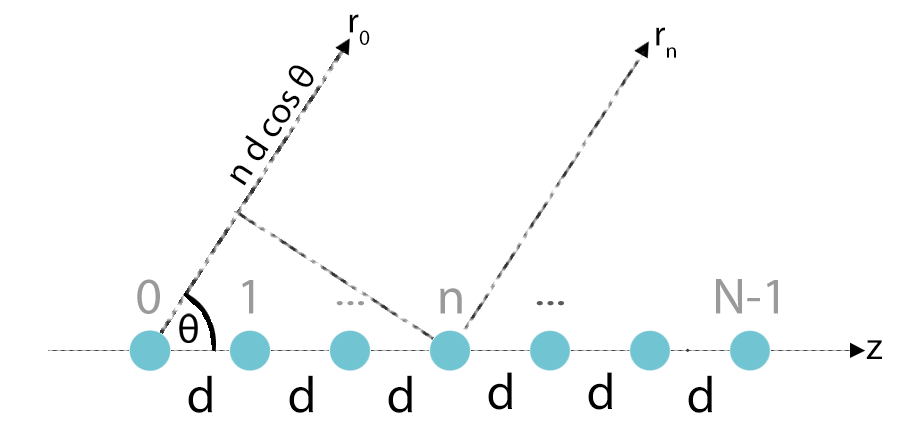
\includegraphics[width=0.65\textwidth]{archivos/array/array}
        \caption{Agrupación lineal de antenas sobre el eje Z.}
        \label{fig:arraigo}
\end{figure}

\begin{equation}
	\vec{J}\left ( \vec{r} \right )=\sum_{n=0}^{N-1}I_{n}\vec{J}_{0}(r-nd\hat{z})
	\label{eq:distrib}
\end{equation}

\par Se puede expresar el sumatorio anterior como la convolución entre la corriente que alimenta un elemento básico del array, es decir, una antena simple, y un tren de deltas ponderadas con sus respectivos pesos $I_{n}$ \cite{Cardama2002}.

\begin{equation}
	\vec{J}\left ( \vec{r} \right )=\vec{J}_{0}\left ( \vec{r} \right ) \ast \sum_{n=0}^{N-1}I_{n}\delta (r-nd\hat{z})=\vec{J}_{0}\left ( \vec{r} \right )\ast I(n)
	\label{eq:conv}
\end{equation}

\par Sabiendo que el vector de radiación $\vec{N}\left ( \vec{r} \right )$, es la transformada de Fourier tridimensional de la distribución de corrientes $\vec{J}\left ( \vec{r} \right )$, se aplicará el teorema de convolución para calcularlo \cite{Cardama2002}.

\begin{equation}
	\vec{N}\left ( \vec{r} \right )=TF_{3D}\left [\vec{J}\left ( \vec{r} \right )  \right ]=\vec{N}_{0}\left ( \vec{r} \right )\cdot TF_{3D}\left [ I(n)   \right ]
	\label{eq:3d}
\end{equation}

\par Donde $\vec{N}_{0}\left ( \vec{r} \right )$ es el vector de radiación del elemento simple situado en el origen, cuando el fasor de alimentación toma el valor unidad. Dado que el fasor de corriente $I_{n}$  es separable, su $TF_{3D}$ consistirá en el producto de las transformadas en cada dirección \cite{Cardama2002}.


\begin{equation}
	TF_{3D}\left [ I(n)   \right ]= TF_{x}\left [ I(n)   \right ]\cdot TF_{y}\left [ I(n)   \right ]\cdot TF_{z}\left [ I(n)   \right ] = TF_{z}\left [ I(n)   \right ] = \sum_{n=0}^{N-1}I_{n} e^{j\omega _{z}n}
	\label{eq:direccional}
\end{equation}

\par Donde $\omega _{z}$ es la frecuencia digital en la dirección del eje $z$, que puede ser obtenida mediante el producto de la frecuencia espacial analógica $k_{z}$  por el periodo de muestreo en la dirección z, que equivale a la distancia de espaciación entre las antenas que componen el array, $d$ \cite{Cardama2002}. 

\begin{equation}
	\omega_{z} = k_{z}\cdot d = k d \cos {\theta } 
	\label{eq:frecdigital}
\end{equation}

\par Donde $\theta$ representa el ángulo cualquiera con respecto a la agrupación de antenas. Teniendo en cuenta que los fasores de alimentación $I_{n}$, presentan una fase progresiva entre cada par de antenas consecutivas que puede expresarse mediante \cite{Cardama2002}: 

\begin{equation}
	I_{n}=a_{n}e^{jn\alpha} 
	\label{eq:fasor}
\end{equation}

\par Donde $a_{n}$ son coeficientes, generalmente complejos, y que pueden tomar valores reales cuando la fase de alimentación sea progresiva, se podrá entonces
obtener el vector de radiación del conjunto de antenas \cite{Cardama2002}:

\begin{equation}
	\vec{N}\left ( \vec{r} \right )= \vec{N}_{0}\left ( \vec{r} \right )\sum_{n=0}^{N-1}a_{n}e^{jn(kd\cos\theta+\alpha)}
	\label{eq:vecrad}
\end{equation}

\par Para simplificar los cálculos, agruparemos el término $kd\cos\theta+\alpha$ en una sola variable, la cual representará la diferencia de fase entre las contribuciones en el campo lejano de dos antenas consecutivas \cite{Cardama2002}. 

\begin{equation}
	\Psi = kd\cos\theta+\alpha
	\label{eq:psi}
\end{equation}

\par Esta diferencia de fase es igual a la suma del desfase por diferencia de caminos $kd\cos\theta$, más la diferencia de fase que progresivamente ha ido alimentando cada antena $\alpha$. Quedando entonces el vector de radiación como \cite{Cardama2002}: 

\begin{equation}
	\vec{N}\left ( \vec{r} \right )= \vec{N}_{0}\left ( \vec{r} \right )\sum_{n=0}^{N-1}a_{n}e^{jn\Psi}
	\label{eq:vecrad2}
\end{equation}

\par Se puede observar cómo el vector de radiación consiste en el producto entre el vector de radiación de la primera antena básica $\vec{N}_{0}\left ( \vec{r} \right ) $ y un factor que tiene en cuenta la interferencia de las \textit{N} ondas generadas por cada antena. Este factor depende unicamente de la separación entre elementos, su alimentación y la frecuencia de trabajo, y se le denomina \textit{factor de agrupación} o \textit{factor de array} (\textit{FA}) \cite{Cardama2002}.

\begin{equation}
	FA(\Psi)=\sum_{n=0}^{N-1}a_{n}e^{jn\Psi}
	\label{eq:fa}
\end{equation}

\section{Factor de array}
\label{FA}
\par Mediante el factor de array se puede obtener el patrón de radiación producido por cualquier array de antenas isotrópicas. Si las antenas que conforman el array no fuesen isotrópicos, se podrá obtener el campo radiado total multiplicando el factor de array por el campo radiado de un elemento único. Cada array tiene su propio factor de array. El factor de array, por lo general, queda en función del número de elementos, su disposición geométrica, sus magnitudes relativas, sus fases relativas, y la distancia entre los elementos \cite{Balanis2015}. 
\\
\par El factor de array presenta las siguientes propiedades \cite{Cardama2002}:

\begin{itemize}
\item \textbf{Periodicidad: }Se trata de una función periódica del ángulo $\Psi$ con periodo $2\pi$, tal que los coeficientes de su serie de Fourier son los coeficientes de la alimentación $a_{n}$. Gracias a esta propiedad se podrá realizar una sintetización de un patrón de radiación mediante el ajuste de los coeficientes de Fourier del factor de array de la agrupación concreta.

\item \textbf{Relación con la TF: }El factor de array puede ser definido ahora como la transformada de Fourier de la secuencia discreta de los coeficientes de la alimentación, $a_{n}$.

\item \textbf{Máximo del factor de array: }Si los coeficientes de la alimentación $a_{n}$ son reales y positivos, el máximo del factor de la agrupación se encuentra en el origen $\Psi=0$. Sabiendo que el máximo del diagrama de radiación se encuentra en la dirección en la que los máximos de cada antena se interfieren positivamente en el espacio, es decir, en fase, la cual corresponde a un desfase nulo ($\Psi=0$) en la interferencia cuando los coeficientes son reales y positivos.

\item \textbf{Margen visible: }Dado que el ángulo $\theta$ solo tomará valores reales entre 0 y $\pi$, se puede deducir el rango de valores de $\Psi$ para los que este fenómeno toma lugar:

\begin{equation}
	\Psi \in \left [ -kd+\alpha ,\; kd+\alpha \right ]
	\label{eq:dominio}
\end{equation}

\par Solamente el intervalo comprendido en (\ref{eq:dominio}) pertenece al diagrama de radiación, lo que se conoce como \textit{margen visible} (fig. \ref{margenvisible}). La longitud del margen visibles es de $2kd$ y está centrado en $\Psi=\alpha$, de forma que su tamaño es proporcional al espaciado de la agrupación, normalizado respecto a la longitud de onda y su posición en el eje $\Psi$ varía con la fase progresiva.

\item \textbf{Máximo del diagrama de radiación: }Cuando los coeficientes de la alimentación son reales y positivos y si el margen visible incluye el origen $\Psi=0$, el máximo del diagrama de radiación se encuentra en $\theta_{max}$. 

 \begin{equation}
	\theta_{max}=\arccos(-\frac{\alpha}{kd}),\ \ \left | \alpha \right |\leq kd
	\label{eq:radmax}
\end{equation}

\par Si se varía la fase de alimentación progresiva $\alpha$, sería posible controlar la dirección del máximo de radiación. Este es el principio de funcionamiento de los \textit{Phased arrays}, en las que la dirección del máximo se varía de forma electrónica mediante un control de la fase relativa progresiva de alimentación de los elementos individuales del array. 

\textbf{Periodicidad de los máximos: }Si el máximo de radiación se encuentra en $\Psi_{max}$ existirán máximos periódicos en los múltiplos enteros de $2\pi$. Cuando estos máximos se encuentran dentro del margen visible:

\begin{equation}
	kd+\alpha\geq 2\pi,\ \
-kd+\alpha\leq 2\pi  
\label{eq:maxdominio}
\end{equation}


\par Aparecerán múltiples máximos de radiación en el espacio real, denominados \textit{lóbulos de difracción} o \textit{grating lobes}. Este fenómeno suele darse cuando el espaciado es de una o más longitudes de onda.
\begin{figure}[h]
    \centering
        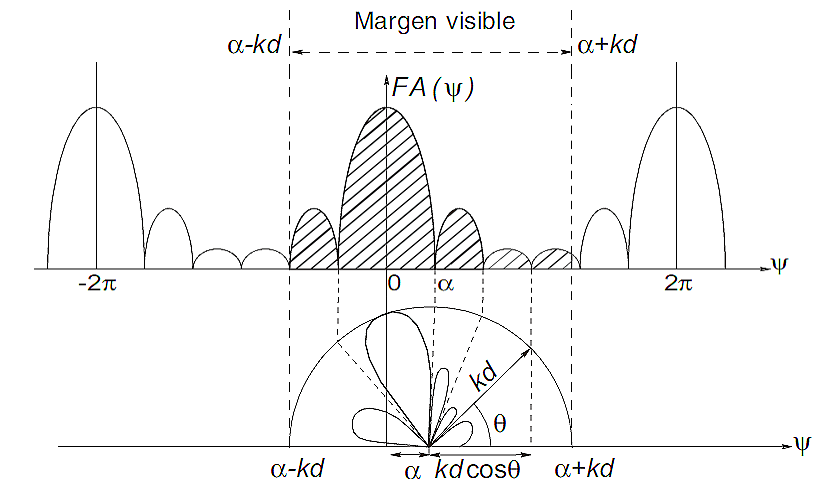
\includegraphics[width=0.62\textwidth]{archivos/array/margen}
        \caption{Margen visible. \cite{Cardama2002}}
        \label{fig:margenvisible}
\end{figure}

\end{itemize}



\newpage
\section{Influencia de los parámetros de diseño}
\par A continuación, se van a realizar un breve resumen sobre los principales efectos que producen sobre el patrón de radiación la modificación de los parámetros de diseño del array, tales como el número de elementos que lo componen, la distancia entre ellos, o el efecto que produciría un desfase relativo en su alimentación. Para la simulación de los efectos deseados se usará el Applet diseñado por Amanogawa para la simulación de arrays uniformes \cite{Amanogawa2019}.

\subsection{Número de elementos}
\par En primer lugar se comenzará variando el número de elementos que componen el array de dipolos uniformes. La configuración del array se basará en la adición de dipolos de longitud $\lambda/2$, alimentados con la misma fase relativa y separados a una distancia entre $\lambda/4$ y $\lambda$ para poder ver cómo la separación entre elementos también afecta a la forma inicial del patrón de radiación.
\\
\par En la tabla \ref{tab:numeroelementos} se puede observar cómo, dado un espacio constante y un aumento del número de elementos del array, la directividad del patrón de radiación va aumentando, y con ello, el número de lóbulos laterales. Se ha de llegar a un compromiso entre la directividad que se desea conseguir en el patrón de directividad final frente al número de lóbulos laterales y la intensidad de estos, a la hora de diseñar un array lineal.


\begin{table}[p]
\centering
\begin{tabular}{ccc}
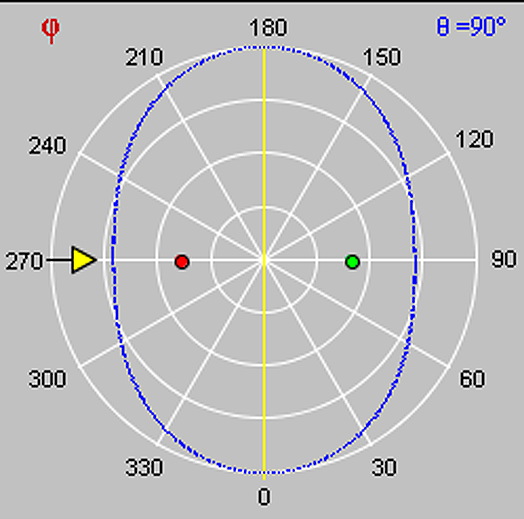
\includegraphics[scale=0.25]{archivos/array/numero/1a} & 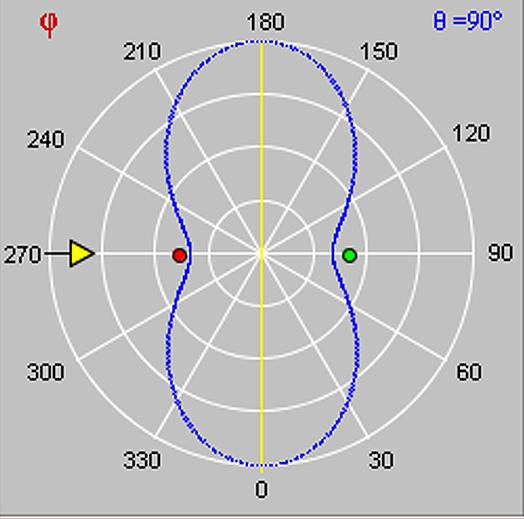
\includegraphics[scale=0.25]{archivos/array/numero/1b} & 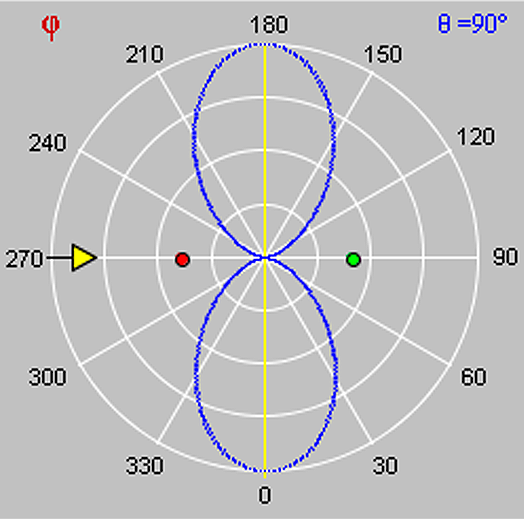
\includegraphics[scale=0.25]{archivos/array/numero/1c} \\
$d=\lambda/4 \; ; \; N=1$  & 
$d=\lambda/4 \; ; \; N=2$  & 
$d=\lambda/4 \; ; \; N=3$  \\

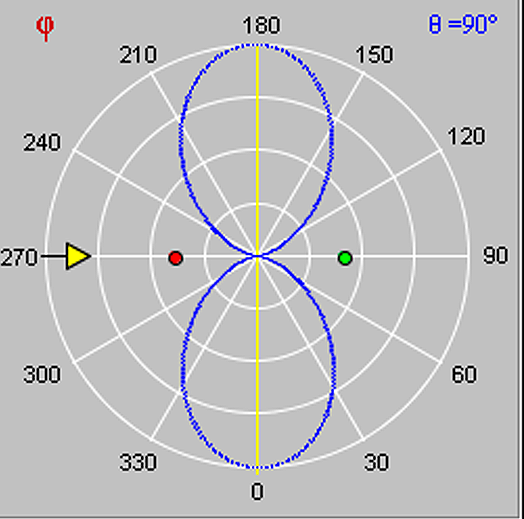
\includegraphics[scale=0.25]{archivos/array/numero/2a} & 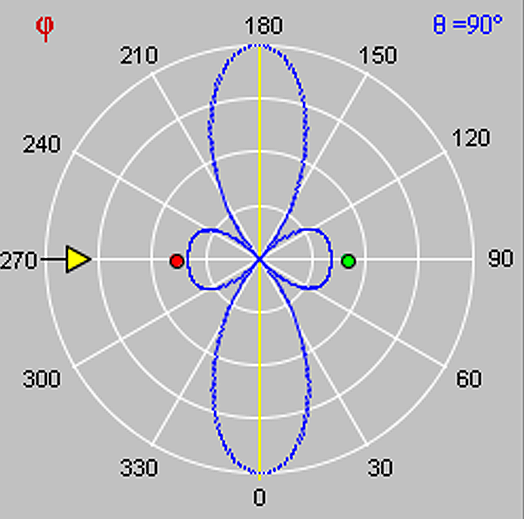
\includegraphics[scale=0.25]{archivos/array/numero/2b} & 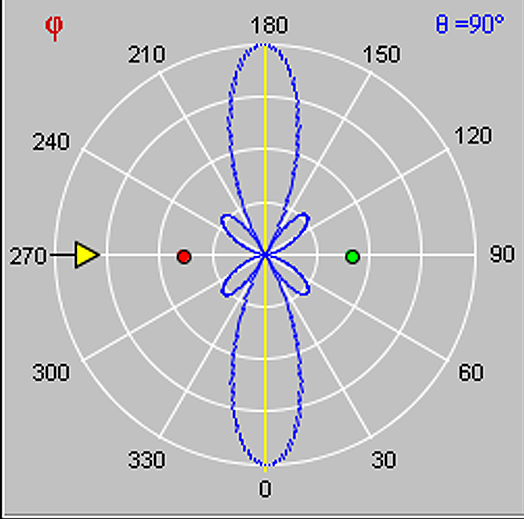
\includegraphics[scale=0.25]{archivos/array/numero/2c} \\
$d=\lambda/2 \; ; \; N=1$  & 
$d=\lambda/2 \; ; \; N=2$  & 
$d=\lambda/2 \; ; \; N=3$  \\

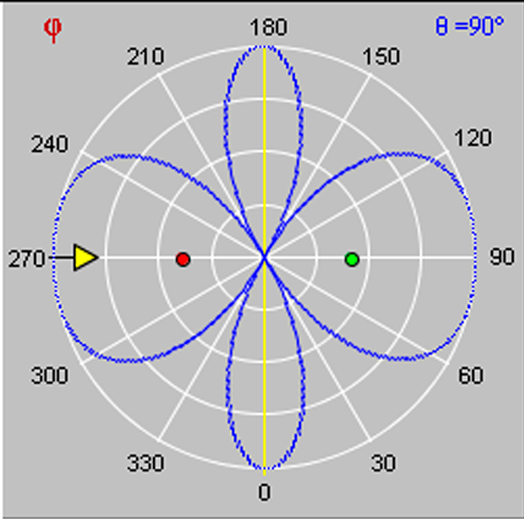
\includegraphics[scale=0.25]{archivos/array/numero/3a} & 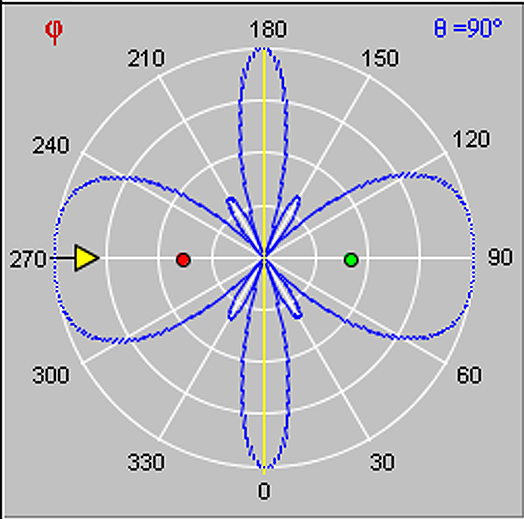
\includegraphics[scale=0.25]{archivos/array/numero/3b} & \includegraphics[scale=0.25]{archivos/array/numero/3c} \\
$d=\lambda \; ; \; N=1$  & 
$d=\lambda \; ; \; N=2$  & 
$d=\lambda \; ; \; N=3$  \\
\end{tabular}
\caption{Efecto de adición de elementos sobre array lineal.}
\label{tab:numeroelementos} % 
\end{table}

\begin{table}[p]
\centering
\begin{tabular}{ccc}
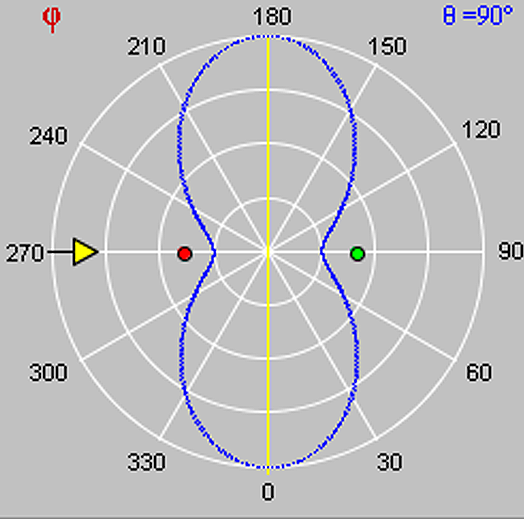
\includegraphics[scale=0.25]{archivos/array/distancia/1a} & 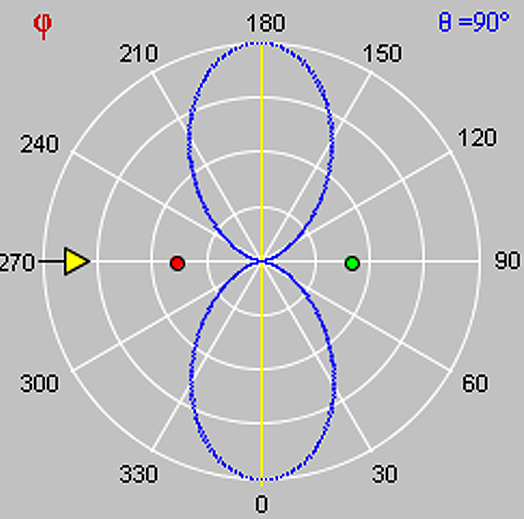
\includegraphics[scale=0.25]{archivos/array/distancia/1b} & 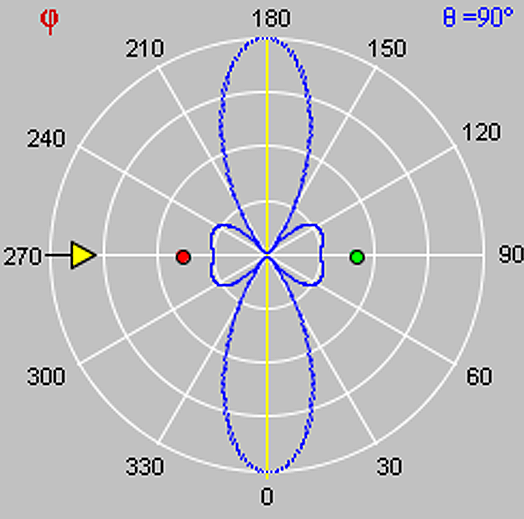
\includegraphics[scale=0.25]{archivos/array/distancia/1c} \\
$d=0.2\lambda$  & 
$d=0.25\lambda$  & 
$d=0.4\lambda$  \\

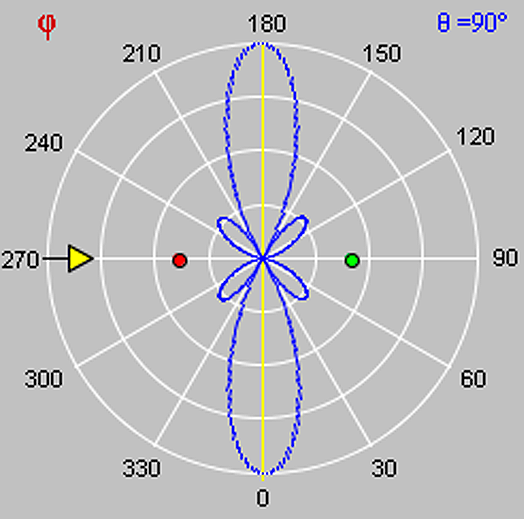
\includegraphics[scale=0.25]{archivos/array/distancia/2a} & 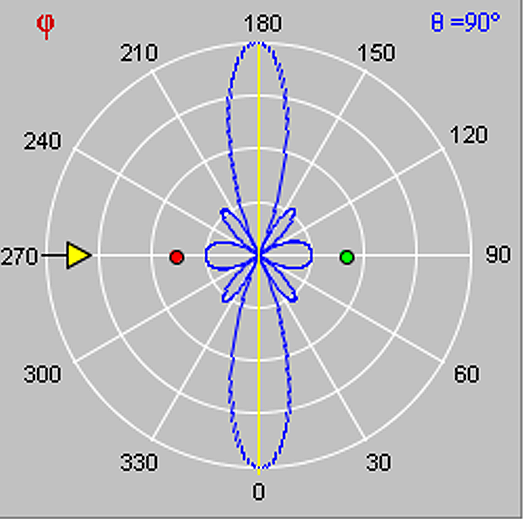
\includegraphics[scale=0.25]{archivos/array/distancia/2b} & 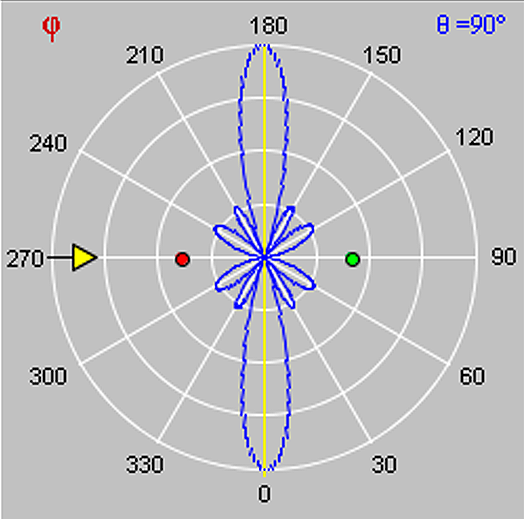
\includegraphics[scale=0.25]{archivos/array/distancia/2c} \\
$d=0.5\lambda$  & 
$d=0.6\lambda$  & 
$d=0.75\lambda$  \\

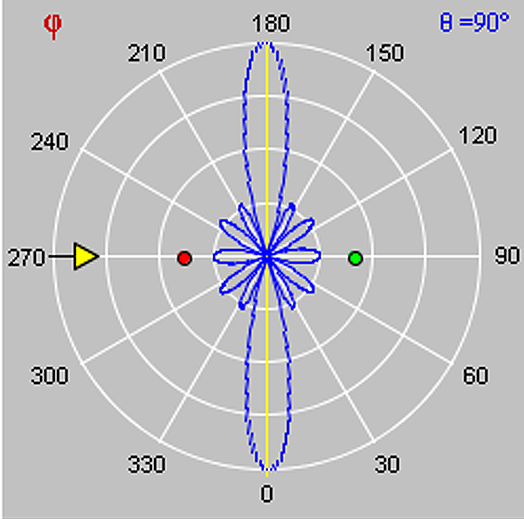
\includegraphics[scale=0.25]{archivos/array/distancia/3a} & 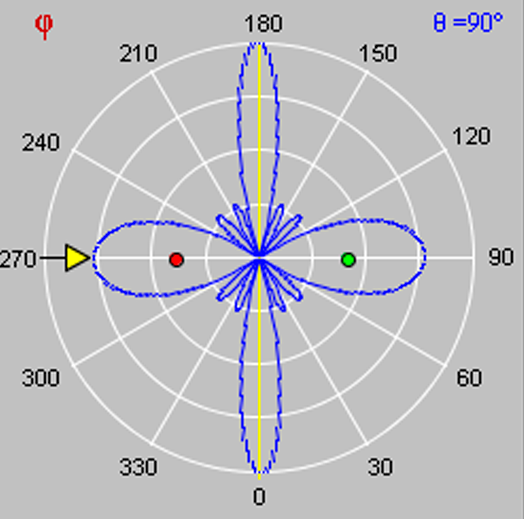
\includegraphics[scale=0.25]{archivos/array/distancia/3b} & \includegraphics[scale=0.25]{archivos/array/distancia/3c} \\
$d=0.8\lambda$  & 
$d=0.9\lambda$  & 
$d=\lambda$  \\
\end{tabular}
\caption{Efecto de la separación de elementos sobre array lineal.}
\label{tab:distanciaelementos} % 
\end{table}




\begin{table}[p]
\centering
\begin{tabular}{ccc}
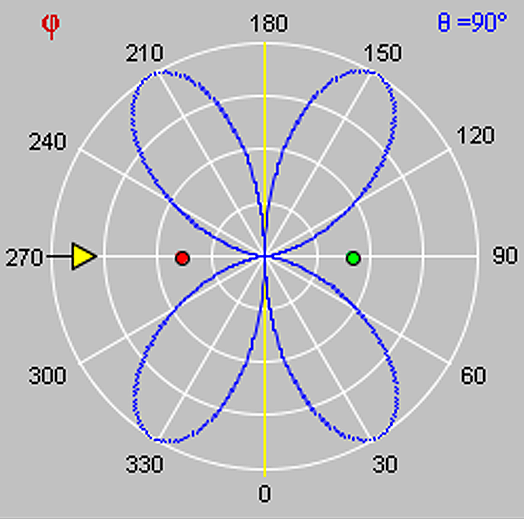
\includegraphics[scale=0.25]{archivos/array/fase/1a} & 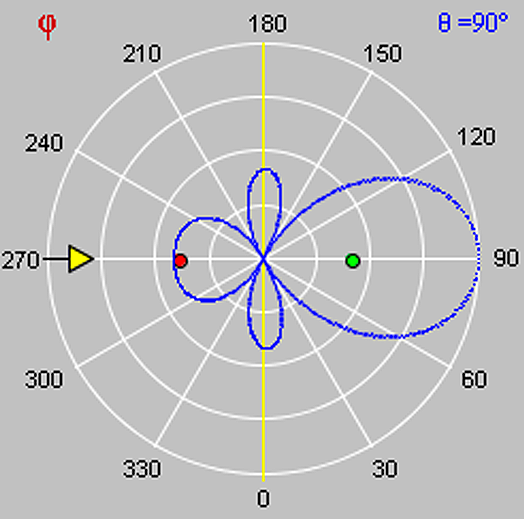
\includegraphics[scale=0.25]{archivos/array/fase/1b} & 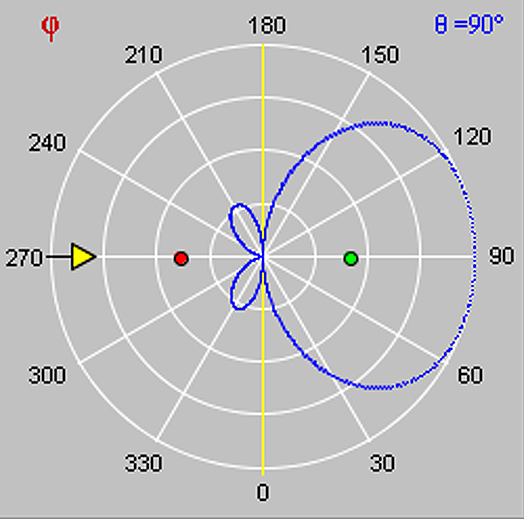
\includegraphics[scale=0.25]{archivos/array/fase/1c} \\
$\alpha=-180^{\circ}$  & 
$\alpha=-135^{\circ}$  & 
$\alpha=-90^{\circ}$  \\

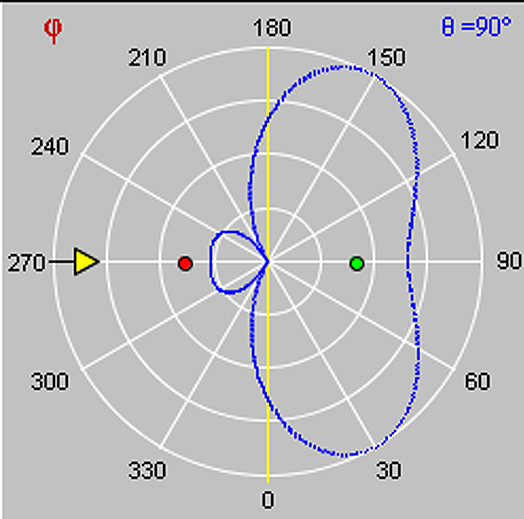
\includegraphics[scale=0.25]{archivos/array/fase/2a} & 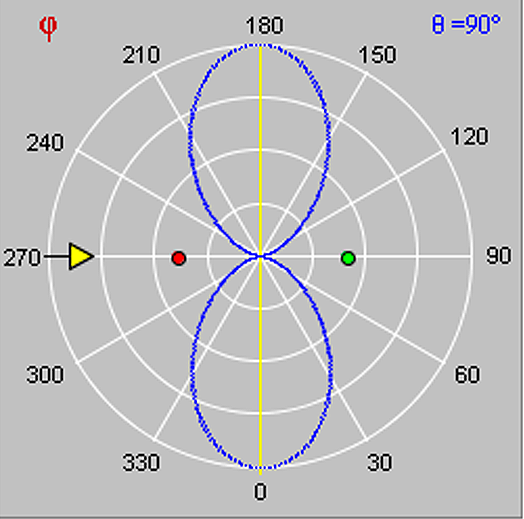
\includegraphics[scale=0.25]{archivos/array/fase/2b} & 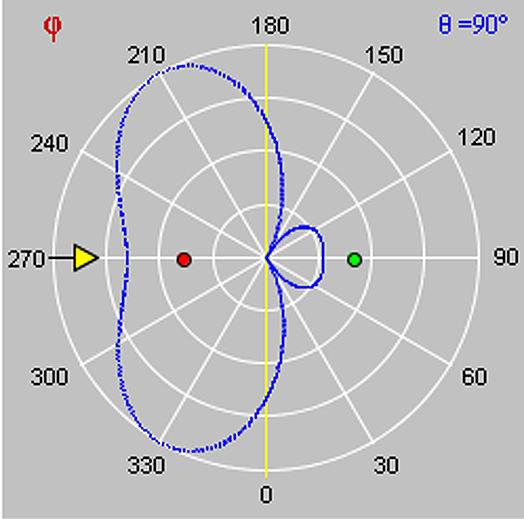
\includegraphics[scale=0.25]{archivos/array/fase/2c} \\
$\alpha=-45^{\circ}$  & 
$\alpha=0^{\circ}$  & 
$\alpha=45^{\circ}$  \\

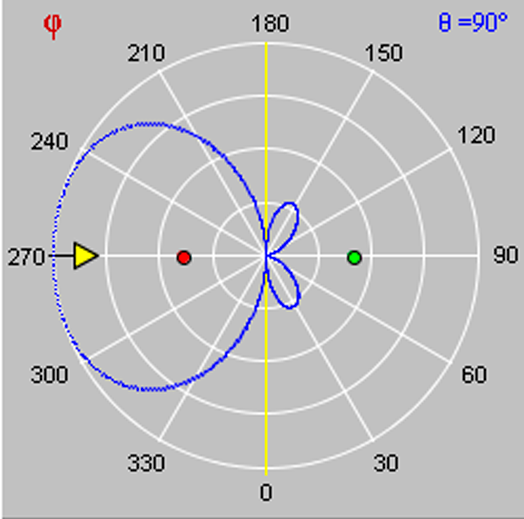
\includegraphics[scale=0.25]{archivos/array/fase/3a} & 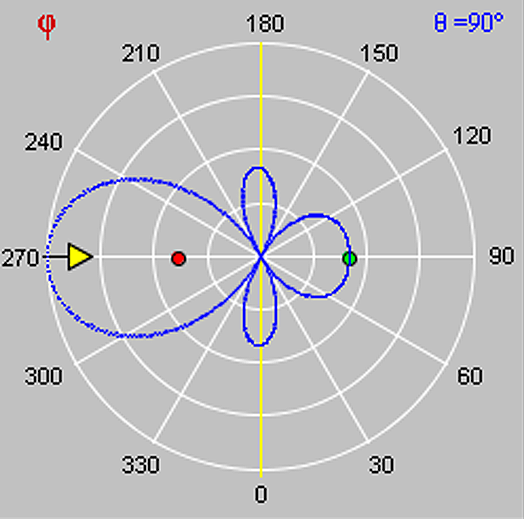
\includegraphics[scale=0.25]{archivos/array/fase/3b} & 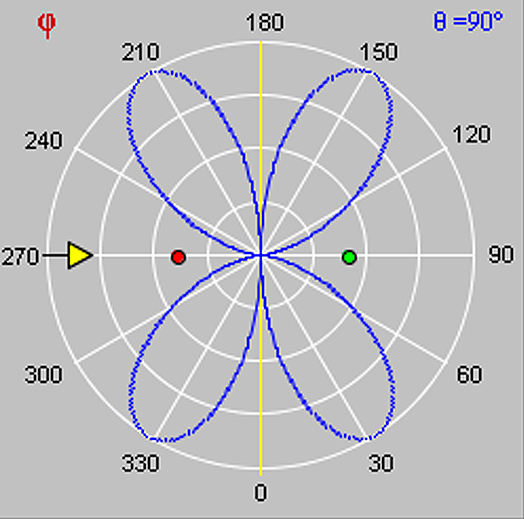
\includegraphics[scale=0.25]{archivos/array/fase/3c} \\
$\alpha=90^{\circ}$  & 
$\alpha=135^{\circ}$  & 
$\alpha=180^{\circ}$  \\
\end{tabular}
\caption{Efecto del desfase de alimentación de los elementos sobre array lineal.}
\label{tab:faseelementos} % 
\end{table}


\subsection{Espaciado de elementos}
\label{espaciado}
\par En esta caso se modificará la separación entre antenas fijando el número de elementos que componen el array a 4 dipolos $\lambda/2$. La principal variación que se observa cuando se aumenta la distancia entre elementos es la aparición de nuevos máximos. 
\\
\par Cuando la distancia de separación es menor a $\lambda/2$ tan solo aparece un máximo principal. Conforme la separación aumenta de $\lambda$ encontraremos la aparición de nuevos máximos principales, como ocurre en la tabla \ref{tab:distanciaelementos} cuando $d=\lambda$. Entre $\lambda/4$ y $\lambda$ encontramos aparición de lóbulos laterales. \cite{Valero2008}






\subsection{Desfase progresivo}
\label{desfasprog}
\par En este último caso, se modificará el desfase progresivo entre las antenas de $-180^{\circ}$ a $+180^{\circ}$, manteniendo, como en las configuraciones anteriores, un array de 4 dipolos $\lambda/2$ separados a una distancia de $\lambda/4$. \cite{Valero2008}
\\
\par Como se puede comprobar en la tabla \ref{tab:faseelementos}, gracias al efecto producido por el desfase en los dipolos se pueden llegar a conseguir patrones de radiación desde \textit{broadside} hasta \textit{end-fire}. Este es es principio de funcionamiento de los \textit{phased arrays}. Esta capacidad de reconfigurabilidad de las antenas es especialmente útil en antenas donde el sujeto no está fijo y se necesita una gran directividad para desperdiciar la mínima energía posible en la radiación.



\newpage
\section{Tipos de agrupaciones}
\par A lo largo de esta sección se realizará un repaso a los principales tipos de agrupaciones usadas para el diseño de arrays de antenas y se hará mención a las características que definen las agrupaciones así como las principales ventajas y aplicaciones de cada una. Definiremos dos tipos principales de agrupaciones según su tipo de distribución en el espacio: unidimensionales, todos los elementos se sitúan a lo largo de un eje común, y bidimensionales, los elementos se sitúan a lo largo de un plano común.

\subsection{Polinomio de agrupación}
\par En la sección \ref{FA} se ha definido y resumido las principales características del factor de array, siendo interpretado como la transformada de Fourier de la secuencia de alimentaciones $a_{n}$. De la misma manera, se puede definir el \textit{polinomio de agrupación} como la transformada Z de la misma secuencia. \cite{Cardama2002}

\begin{equation}
	P(z)=\sum_{n=0}^{N-1}a_{n}z^{n}=a_{0}+a_{1}z+a_{2}z^{2}+...+a_{N-1}z^{N-1}
	\label{eq:z}
\end{equation}

\par El polinomio de agrupación se relaciona con la factor de agrupación mediante:


\begin{equation}
	FA(\Psi)=P(z)|_{z=e^{j\Psi}}
	\label{eq:faz}
\end{equation}

\par Con esto se deduce que el factor de agrupación corresponde al polinomio de agrupación de un array concreto pero muestreado sobre la circunferencia unidad. Cada periodo de $2\pi$ en $\Psi$ del factor de agrupación corresponde a una vuelta sobre el círculo unidad en el plazo $Z$. El diagrama de radiación del array está asociado al intervalo del círculo unidad definido por el margen visible. Como los ceros del polinomio que están situados sobre el circulo unidad  y dentro del margen visible corresponden a nulos del diagrama de radiación, se puede aproximar la forma del diagrama de radiación a partir de la posición de los ceros en el plano $Z$. \cite{Cardama2002}

\subsection{Agrupaciones unidimensionales}
\par En primer lugar se hará un resumen de las principales agrupaciones unidimensionales y sus características. Como se ha mencionado, las agrupaciones unidimensionales son aquellas en las cuales los elementos que componen la agrupación se sitúan a lo largo de un mismo eje. Dentro de las configuraciones unidimensionales, podemos clasificar tres tipos principales de distribución de corrientes: uniformes, triangulares y binómicas. \cite{Cardama2002}
\\
\par El nombre que reciben este tipo de configuraciones viene dado, no por la distribución de las antenas en el espacio, sino por la distribución de los ceros en el polinomio de agrupación en el círculo unidad.

\subsubsection{Distribución uniforme}
\par La distribución de corrientes uniforme es aquella en la que se alimentan todos las antenas que componen el array con la misma amplitud de excitación $a_{n}=1$. Su polinomio de agrupación es: \cite{Cardama2002}

\begin{equation}
	P(z)=1+z+z^{2}+...+z^{N-1}=\frac{z^{N}-1}{z-1}
	\label{eq:disuniform}
\end{equation}

\par De esta expresión se puede deducir que los ceros del polinomio de agrupación en el plano Z son las raíces N-ésimas de la unidad salvo $z=1$, y por ello, estos ceros se encuentran equiespaciados sobre el círculo unidad. \cite{Cardama2002}

\begin{figure}[h]
    \centering
        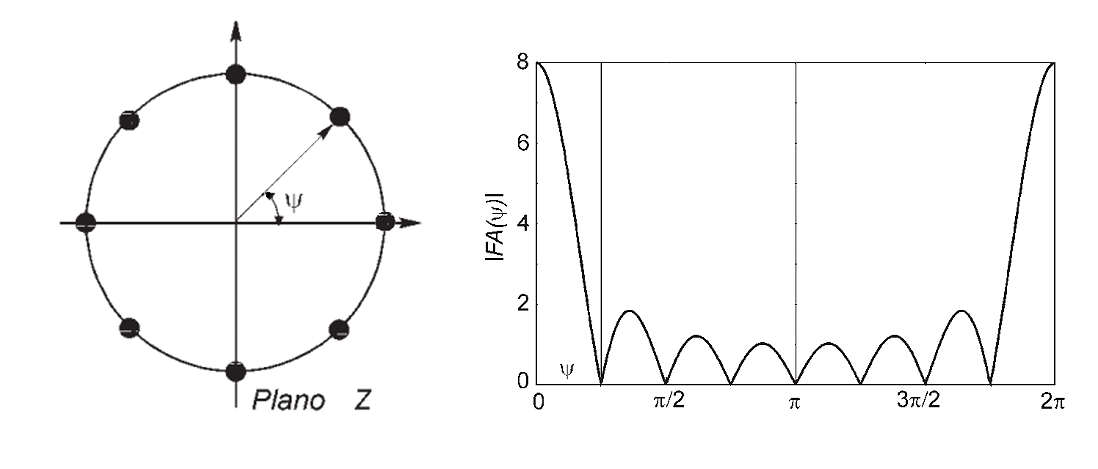
\includegraphics[width=0.8\textwidth]{archivos/array/uniforme}
        \caption{Ceros en el plano Z y en el módulo del \textit{FA} para el caso de un array de 8 elementos y distribución uniforme. \citep{Cardama2002}}
        \label{fig:cerosuniforme}
\end{figure}

\par Teniendo en cuenta las ecuaciones \ref{eq:faz} y \ref{eq:disuniform} se puede deducir el factor de agrupación, obteniéndose: \cite{Cardama2002}

\begin{equation}
	\left | FA (\Psi) \right |=\frac{\left | e^{jN\Psi}-1 \right |}{\left | e^{j\Psi}-1 \right |}
	\label{eq:casisinc}
\end{equation}

\par Se puede observar que el factor de agrupación obtenido es una función \textit{sinc} periódica, igual a la TF de un pulso muestreado. \cite{Cardama2002}

\subsubsection{Distribución triangular} 
\par La distribución de corrientes triangular se define para un array con un número de elementos impar. La alimentación de estas viene dada por: \cite{Cardama2002}

\begin{equation}
	a_{n}=\begin{cases} n+1, &  n< \frac{N}{2} \\ N-n, & n> \frac{N}{2} \end{cases}
	\label{eq:casotriang}
\end{equation}

\par Si desarrollamos el polinomio Z (eq. \ref{eq:z} y \ref{eq:faz}), y tenemos en cuenta que la función triangular puede descomponerse en la convolución de dos pulsos iguales cuya longitud es la mitad que la del triángulo, lo que se traduce en un producto de transformadas en el dominio Z, el polinomio de la distribución de corrientes triangular puede expresarse como: \cite{Cardama2002}

\begin{equation}
	P(z)=1+2z+3z^{2}+...+3z^{N-3}+2z^{N-2}+z^{N-1}=\left [ \frac{z^{\frac{N+1}{2}}-1}{z-1} \right ]^{2}
	\label{eq:casotriangpoli}
\end{equation}

\par Los ceros de la distribución triangular son los mismos que se obtendrían para el caso de la distribución de corrientes uniformes con $(N+1)/2$ antena, pero dobles. El factor de agrupación es también el obtenido para una distribución uniforme de longitud $[(N+1)/2]^{2}$: \cite{Cardama2002}

\begin{equation}
	\left | FA (\Psi) \right |=\frac{\left |  \sin\left ( \frac{N+1}{4}\Psi \right )\right |^{2}}{\left | \sin\left ( \frac{\Psi}{2} \right ) \right |^{2}}
	\label{eq:fa2}
\end{equation}

\begin{figure}[h]
    \centering
        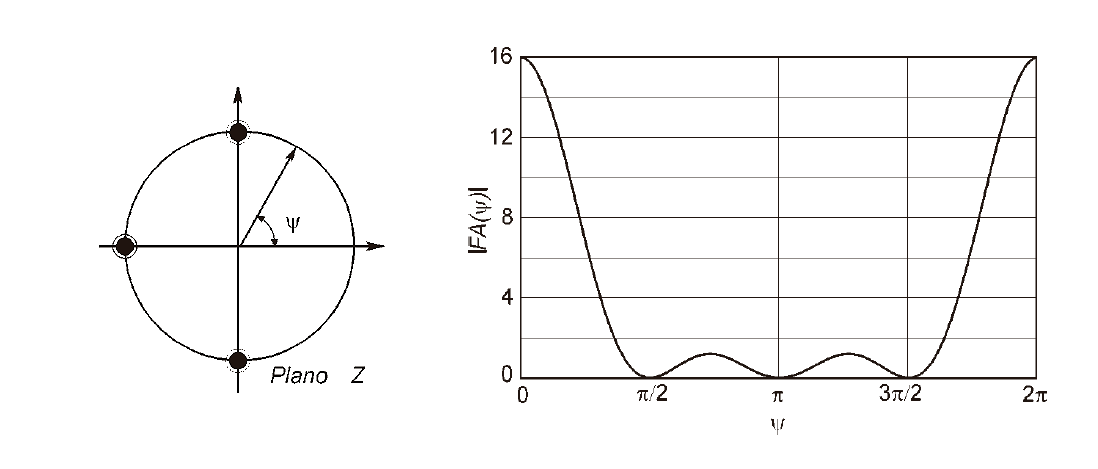
\includegraphics[width=0.8\textwidth]{archivos/array/triangular}
        \caption{Ceros en el plano Z y en el módulo del \textit{FA} para el caso de un array de 7 elementos y distribución triangular. \citep{Cardama2002}}
        \label{fig:cerostrinagular}
\end{figure}

\subsubsection{Distribución binómica}
\par La distribución de corrientes binómica define el polinomio como un binomio elevado a una potencia y desarrollado según la fórmula de Newton: \cite{Cardama2002}

\begin{equation}
	P(z)=(z+1)^{N-1}=\binom{N-1}{0}+\binom{N-1}{1}z+\binom{N-1}{2}z^{2}+...+\binom{N-1}{N-1}z^{N-1}
	\label{eq:newton}
\end{equation}

\par Los coeficientes de excitación del polinomio de agrupación se pueden obtener a través de la expresión de números combinatorios. \cite{Cardama2002}

\begin{equation}
	a_{n}=\binom{N-1}{n}=\frac{\left ( N-1 \right )!}{n!\left ( N-1-n \right )!}
	\label{eq:combinatorios}
\end{equation}

\par El polinomio de la distribución de corrientes binómica presenta un solo cero, situado en $\Psi=\Pi$ y con multiplicidad $N-1$. Es por ello que el ancho de haz entre ceros de $\Psi$ es de $2\pi$ y no existen lóbulos secundarios en el módulo del factor de agrupación. Sin embargo, en el patrón de radiación si pueden aparecer lóbulos secundarios debido a la los lóbulos de difracción, que entra en el margen visible. El factor de agrupación obtenido para esta distribución es: \cite{Cardama2002}

\begin{equation}
	\left | FA (\Psi) \right |=\left | 2\cos\frac{\Psi}{2} \right |^{N-1}	
	\label{eq:Fabinom}
\end{equation}

\begin{figure}[h]
    \centering
        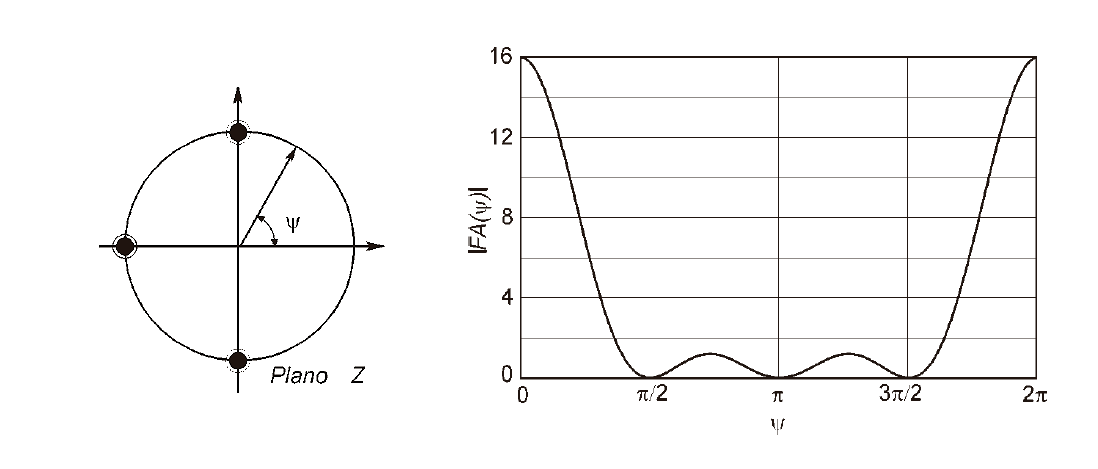
\includegraphics[width=0.8\textwidth]{archivos/array/triangular}
        \caption{Ceros en el plano Z y en el módulo del \textit{FA} para el caso de un array de 8 elementos y distribución binómica. \citep{Cardama2002}}
        \label{fig:cerosbinom}
\end{figure}


\subsection{Agrupación lineal uniforme}
\par La agrupación lineal uniforme es aquella en la que los elementos que componen el array están equiespaciados y excitados con la misma amplitud. Se trata de una configuración muy usada y estudiada. Este tipo de agrupaciones también tiene utilidad en aplicaciones de acústica, donde las antenas serían sustituidas por micrófonos o altavoces para lograr mayores ganancias. En el caso de las antenas, las características de la agrupación lineal uniforme son básicas para el diseño de aplicaciones RADAR. 
\\
\par Se va a mencionar dos tipos de configuraciones lineales uniformes según el tipo de patrón de radiación que se desea obtener en el diseño final. En la sección \ref{desfasprog} se hizo mención a los conceptos \textit{broadsire} y \textit{endfire}. Estos conceptos definen los casos en los que el máximo de radiación sea transversal (\textit{broadsire}) o longitudinal (\textit{endfire}) con respecto al eje de la agrupación. \cite{Cardama2002}

\subsubsection{Agrupaciones transversales}

\par Las configuración transversal o \textit{broadsire} es muy usada en aplicaciones que requiere un máximo de radiación en el eje normal al array ($\theta_{0}=90^{\circ}$). Para conseguir este resultado se debe diseñar el array tal que el máximo de radiación de un solo elemento así como el máximo de radiación del factor de array deben dirigirse a $\theta_{0}=90^{\circ}$. \cite{Balanis2015} 
\\
\par Para conseguir que el máximo de radiación de un solo elemento radie en esta dirección basta con saber elegir qué elemento radiante es el mejor para nuestro sistema. Por otro lado, para conseguir que el factor de array tenga un máximo en $\theta_{0}=90^{\circ}$, se deberá ajustar correctamente la separación y la fase de excitación de los elementos del array. Se tomará como punto de partida la ecuación \ref{eq:psi}, en la que buscaremos un nulo (máximo de radiación). \cite{Balanis2015} 

\begin{equation}
	\Psi=kd\cos\theta+\alpha=0
	\label{eq:nulo}
\end{equation}

\par De donde obtenemos $\alpha$ como: 

\begin{equation}
	\Psi=kd\cos\theta|_{\theta=90^{\circ}} +\alpha\rightarrow  \alpha=0
	\label{eq:alphita}
\end{equation}

\par De la ecuación \ref{eq:alphita} se deduce que, para que el factor de array tenga un máximo en $\theta_{0}=90^{\circ}$, no debe existir ningún desfase a la hora de excitar los elementos del array, así como ninguna diferencia de amplitud en la exitación. Aunque la separación de los elementos puede tomar cualquier valor, para asegurarnos que no existan lóbulos de difracción, esta separación no debe tomar valores múltiplos enteros de la longitud de onda. \cite{Balanis2015}




\subsubsection{Agrupaciones longitudinales}

\par Por otro lado tenemos la configuración denominada longitudinal o \textit{end-fire}. En este caso el máximo de radiación se encontrará a lo largo de la dirección del array, y no en la normal de esta, como en el caso \textit{broadside}. Con este tipo de configuraciones es, además, posible conseguir que solo exista el máximo en una dirección, ya sea a $\theta_{0}=0^{\circ}$ ó $\theta_{0}=180^{\circ}$. Partiendo de la ecuación \ref{eq:psi} buscaremos los máximos $\Psi=0$ para los ángulos de $0^{\circ}$ y $180^{\circ}$.   \cite{Balanis2015}

\begin{equation}
	\Psi = kd\cos\theta+\alpha|_{\theta=0^{\circ}}\rightarrow kd+\alpha=0\rightarrow \alpha=-kd
	\label{eq:end1}
\end{equation}

\begin{equation}
	\Psi = kd\cos\theta+\alpha|_{\theta=180^{\circ}}\rightarrow kd+\alpha=0\rightarrow \alpha=kd
	\label{eq:end2}
\end{equation}

\par Se puede comprobar como para conseguir máximos de radiación en la dirección de $0^{\circ}$ se debe alimentar el array con una fase progresiva de $\alpha=-kd$, y $\alpha=kd$ en el caso de la dirección de $180^{\circ}$. Si la separación de los elementos es de $d=\lambda/2$, se obtendrán máximos de radiación en ambas direcciones. Además, esta separación es múltiplo entero de $\lambda$, se obtendrán máximos tanto en las direcciones de $0^{\circ}$ y $180^{\circ}$ características de la configuración \textit{end-fire} como en las direcciones de
$90^{\circ}$, es decir, de la configuración \textit{broadside}. \cite{Balanis2015}

\begin{figure}[h]
    \centering
        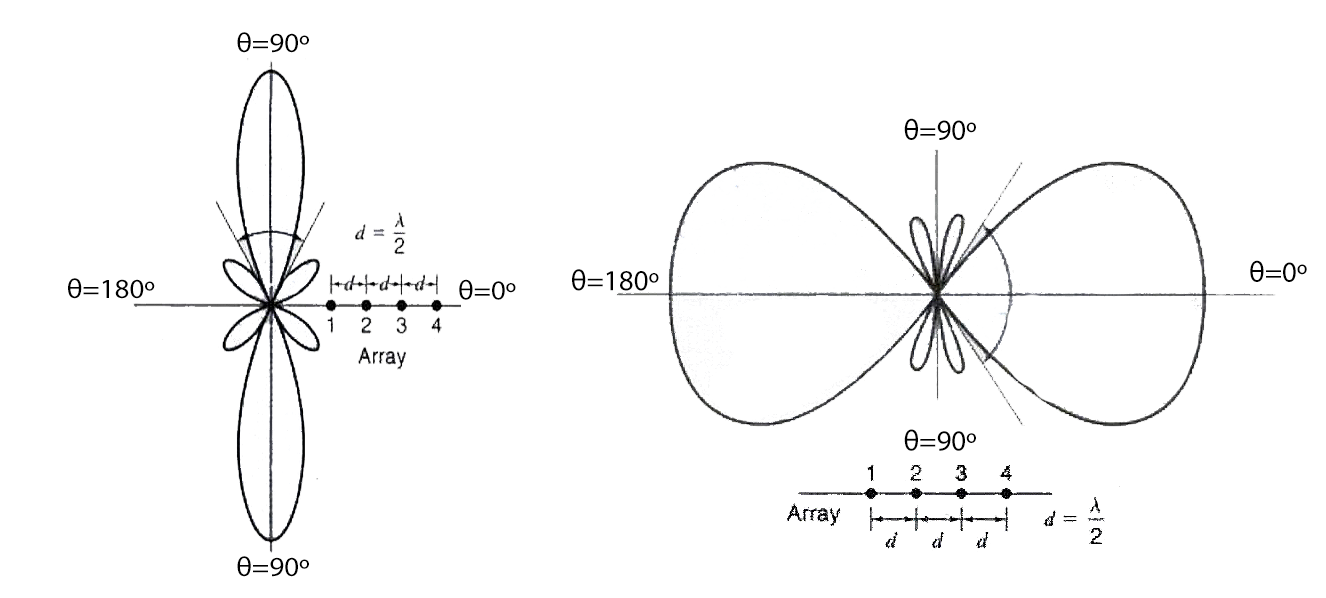
\includegraphics[width=\textwidth]{archivos/array/side}
        \caption{Comparación de radiación \textit{broadside} y \textit{endfire}.}
        \label{fig:side}
\end{figure}

\subsection{Agrupaciones bidimensionales}
\par Las agrupaciones bidimensionales son aquellas en las que los elementos que conforman el array se sitúan sobre un plano común. En las agrupaciones unidimensionales, el diagrama de radiación producido se caracterizaba por tener una simetría de revolución respecto al eje de la agrupación. Las agrupaciones bidimensionales permiten obtener diagramas de radiación más complejos, y brindan la capacidad de dirigir el haz de propagación en las dos coordenadas esféricas del espacio $(\theta, \phi)$, sin las restricciones impuestas por la simetría de revolución. \cite{Cardama2002}
\\
\subsubsection{Agrupación bidimensional uniforme}
\par La agrupación bidimensional más sencilla es la agrupación bidimensional uniforme (fig. \ref{fig:bidimensionalfoto}). Esta configuración se caracteriza por tener una distribución de antenas rectangular a lo largo de un mismo plano, conformada por $MxN$ antenas idénticas, equiespaciadas con separación $d_{x}$ a lo largo del eje $x$ y $d_{y}$ a lo largo del eje $y$, y alimentadas con una corriente $I_{mn}$, es decir, con la capacidad de alimentación individual. \cite{Cardama2002}
\\
\par El factor de agrupación será el resultado de la interferencia en el campo lejano de la radiación de todas las antenas. Por analogía a la ecuación \ref{eq:vecrad}, el factor de agrupación para una agrupación bidimensional uniforme es: \cite{Cardama2002}

\begin{equation}
	FA (k_{x},k_{y}) =\sum_{m=0}^{M-1} \sum_{n=0}^{N-1} I_{mn}e^{jmk_{x}d_{x}}e^{jnk_{y}d_{y}}
	\label{eq:fabinom}
\end{equation}

\par Para una excitación con fase progresiva $\alpha_{x}$ en la dirección $x$ y $\alpha_{y}$ en la dirección $y$. \cite{Cardama2002}

\begin{equation}
	FA (k_{x},k_{y}) =\sum_{m=0}^{M-1} \sum_{n=0}^{N-1} I_{mn}e^{jmk_{x}d_{x}}e^{jnk_{y}d_{y}}
	\label{eq:excitbinom}
\end{equation}

\par Definiendo los ángulos $\Psi_{x}$ y $\Psi_{x}$ como el desfase eléctrico entre las contribuciones en campo lejano de dos elementos consecutivos en los planos $(x,z)$ y $(y,z)$: \cite{Cardama2002}

\begin{equation}
	\begin{matrix}
\Psi_{x}=kd_{x}\sin\theta\cos\phi+\alpha_{x}
 \\
\Psi_{y}=kd_{y}\sin\theta\sin\phi+\alpha_{y}
\end{matrix}
	\label{eq:sinsin}
\end{equation}

\par Resultando el factor de agrupación: \cite{Cardama2002}

\begin{equation}
	FA (\Psi_{x},\Psi_{y}) =\sum_{m=0}^{M-1} \sum_{n=0}^{N-1} a_{mn}e^{jm\Psi_{x}}e^{jm\Psi_{x}}
	\label{eq:fatipo2}
\end{equation}

\begin{figure}[h]
     \centering
     \begin{subfigure}[b]{0.45\textwidth}
         \centering
         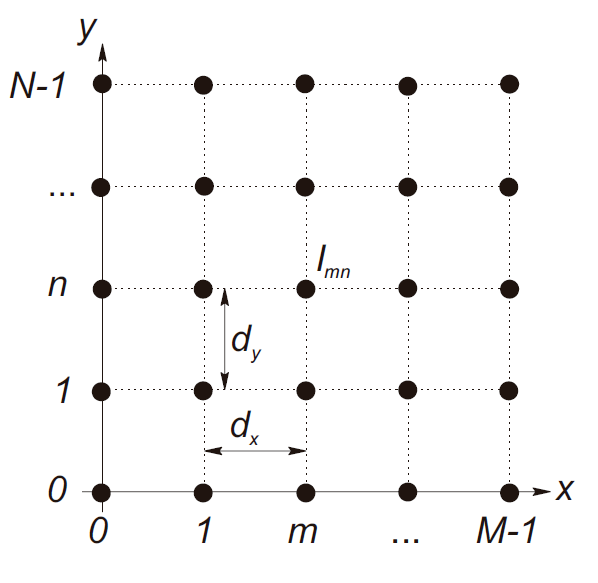
\includegraphics[width=\textwidth]{archivos/array/bidimensional}
         \caption{Representación analítica del array bidimensional uniforme. \cite{Cardama2002}}
         \label{fig:bidimensionalfoto}
     \end{subfigure}
     \hfill
     \begin{subfigure}[b]{0.45\textwidth}
         \centering
         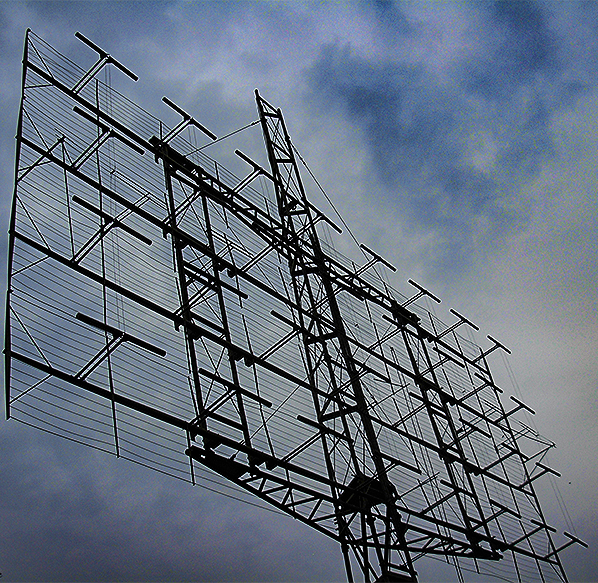
\includegraphics[width=\textwidth]{archivos/array/fotoarray}
         \caption{RADAR basado en array bidimensional. \cite{brewbooks2008} }
         \label{fig:radarfoto}
     \end{subfigure}
     \hfill
\end{figure}

\par Mediante la variación de la longitud de onda $\lambda$, los espaciados eléctricos $d_{x}/\lambda$ y $d_{y}/\lambda$, o las fases progresivas $\alpha_{x}$ y $\alpha_{y}$, se pueden controlar los ángulos $\theta_{max}$ y $\phi_{max}$ para dirigir el haz de máxima radiación en la dirección deseada. También, si se aumenta la distancia de separación hasta superar $\lambda$ se podrán obtener lóbulos de difracción, o \textit{gratin lobes} que podrán actuar como segundos haces en caso de que fuera necesario para la aplicación.
\\
\par En este proyecto, las agrupaciones diseñadas se basan en agrupaciones bidimensionales uniformes, lo que significa que los arrays a diseñar, dispondrán de antenas dispuestas a lo largo de un mismo plano común, y las antenas estarán siempre equiespaciadas con sus antenas colindantes laterales, superiores e inferiores, pero no con las diagonales. 

\section{Alimentación de arrays}
\par Previo al diseño de la antena, es importante conocer qué tipo de alimentación va a usar esta. Cuando se trabaja con agrupaciones de antenas, es importante que todas las antenas estén correctamente interconectadas, así como tener en cuenta los caminos que la señal toma para llegar hasta los diferentes elementos ya que, como se ha mencionado en las secciones anteriores, un pequeño desfase en uno de los elementos, puede modificar por complejo el patrón de radiación inicialmente diseñado para la antena. Por lo general, se pueden categorizar el tipo de alimentación de un array según la forma de interconexión de los diferentes elementos como: alimentación en serie o \textit{series feed} y alimentación en paralelo o \textit{corporate-feed}. 
\\
\par Si nos centramos en el caso de las antenas de parche microstrip, la alimentación en paralelo es comúnmente usada para obtener divisiones de potencia de $2^{n}$, siendo $n$ el número de líneas que se subdividen en paralelo a partir de una sola línea de alimentación. Además, en las líneas de alimentación en paralelo se han de usar o bien líneas de alimentación cónicas (\textit{tapered lines}) que son capaces de mantener su impedancia en las divisiones de caminos, o mediante transformadores $\lambda/4$, cuyo funcionamiento se explicará en la sección \ref{lambdacuartoscap} de este proyecto. \cite{Balanis2015}

\subsection{Líneas de alimentación en serie}
\par En la alimentación en serie de un array de antenas, los elementos  que componen la agrupación son alimentados con la excitación proveniente del elemento anterior (fig. \ref{fig:seriesfeed}). En el caso de las antenas microstrip alimentadas por líneas de alimentación microstrip en serie, estas suelen ser fabricadas usando procesos litográficos tanto para los elementos radiantes como para las líneas de alimentación. Esta técnica limita a la agrupación a poseer unas características radiantes fijadas en su fabricación, ya que no permiten la adición de componentes electrónicos que sean capaz de, por ejemplo, variar la fase progresiva con la que se alimenta cada elemento. \cite{Balanis2015}
\\
\begin{figure}[h]
    \centering
        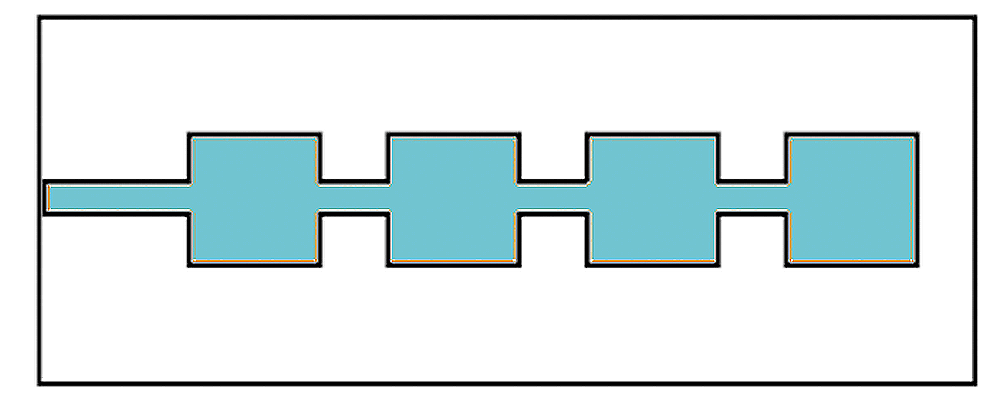
\includegraphics[width=0.65\textwidth]{archivos/array/series}
        \caption{Esquema de interconexión en serie. \cite{Balanis2015}}
        \label{fig:seriesfeed}
\end{figure}

\par Otra opción de reconfigurabilidad de los arrays microstrip en serie es variar la frecuencia de trabajo, lo que puede conducir a diferentes patrones de radiación. Por otro lado, se ha de tener en cuenta que cualquier cambio o imperfección que se produzca sobre cualquiera de los elementos del array así como en cualquier punto de la línea de alimentación, afectará al funcionamiento de la antena, puesto que la excitación de cualquiera de los elementos del array dependerá de sus otros elementos interconectados. \cite{Balanis2015}

\subsection{Líneas de alimentación en paralelo}
\par Las líneas de alimentación interconectadas en paralelo o \textit{corporate-feed} son las más comunes y, por lo general, más versátiles en su uso. Mediante este método el diseñador posee un mayor control sobre la alimentación de cada uno de los elementos de la agrupación. Mediante la variación de la fase y la amplitud de excitación de uno o varios de los elementos del array se pueden llegar a implementar patrones de radiación imposibles de conseguir mediante elementos simples o configuraciones de arrays conectados en serie.
\\
\par La configuración de alimentación en paralelo suele proporcionar un ancho de banda mayor que en el caso de la alimentación en serie y, en algunos casos, mayor que el ancho de banda proporcionado por un solo elemento. Este efecto es principalmente debido a la cancelación de las reflexiones mediante la mayor disipación de potencia producida a lo largo de la red de alimentación. Por todas estas razones, la alimentación en paralelo de parches microstrip es usada en la mayoría de las agrupaciones microstrip, por ejemplo, en las estaciones base de telefonía móvil. \cite{Waterhouse2010}. 

\begin{figure}[p]
    \centering
        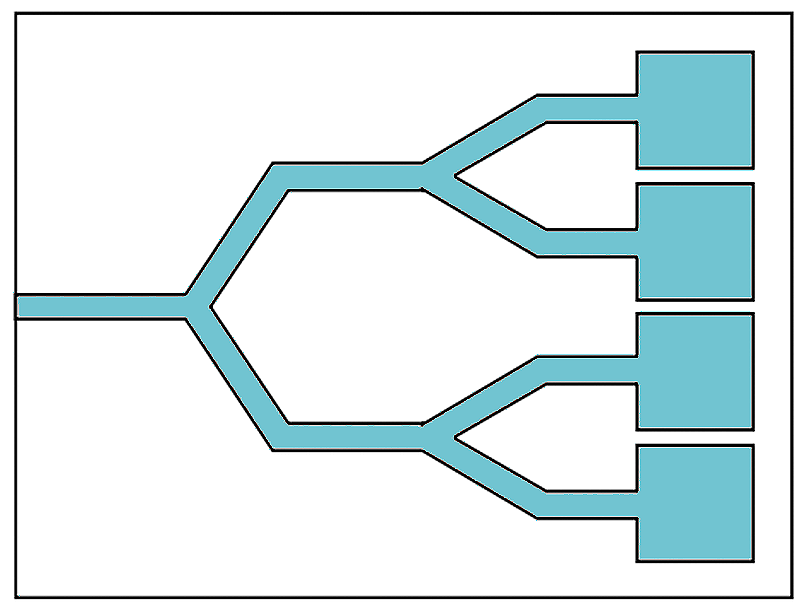
\includegraphics[width=0.7\textwidth]{archivos/array/corporate}
        \caption{Esquema de interconexión en paralelo. \cite{Balanis2015}}
        \label{fig:corporatefeedfeed}
\end{figure}

\begin{figure}[p]
    \centering
        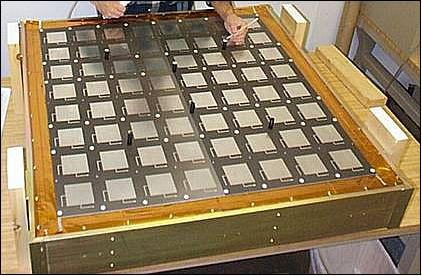
\includegraphics[width=0.7\textwidth]{archivos/array/arrayraro}
        \caption{Esquema de interconexión en paralelo. \cite{NASA2008}}
        \label{fig:nasafoto}
\end{figure}

\section{Separación de elementos}
\par Como se mencionó en la sección \ref{espaciado}, la separación entre los elementos de un array es clave para modelar el patrón de radiación de este. Actualmente existen dos limitaciones principales a la hora de realizar el diseño del array en cuento al parámetro de separación de elementos, la distancia mínima y máxima entre estos.
\\
\par Comenzando con la distancia máxima viable para el diseño, y teniendo en cuenta lo observado en las tabla de imágenes \ref{tab:distanciaelementos}, se evitará que la distancia entre los parches sea mayor a $\lambda_{0}$, para evitar la formación de lóbulos de difracción o \textit{grating lobes}. Por otro lado, la distancia mínima viable viene definida por la limitación en términos de acoplamiento mutuo entre parches, cuyos efectos empiezan a estar presentes en distancias entre $\lambda/4$ y $\lambda/2$.
\\
\par Teniendo en cuenta los límites marcados, y observando las separaciones entre parches que han sido utilizadas en otros diseños publicados \cite{Waterhouse2010, Bertol2017}, se ha decidido usar en todos los diseños realizados, una separación entre los parches del array de $0.7\lambda_{0}$. Esta distancia se tomará de referencia entre los centros de cada antena (fig. \ref{fig:ejemploseparación}). En la tabla \ref{tab:sepparches} se recogen las distancias de separación entre elementos para las tres frecuencias utilizadas en los diseños realizados. 

\begin{table}[H]
   
   \label{tab:sepparches}
   \small % text size of table content
   \centering % center the table
   \begin{tabular}{m{0.4\linewidth}m{0.4\linewidth}} % alignment of each column data
   \toprule[\heavyrulewidth]\toprule[\heavyrulewidth]
   \textbf{Frecuencia} & \textbf{Separación entre elementos}  \\ 
   \midrule
   \textbf{2.4 GHz} & 87.4 mm  \\
   \textbf{6 GHz} & 35 mm  \\
   \textbf{27 GHz} & 7.77 mm  \\
   \bottomrule[\heavyrulewidth] 
   \end{tabular}
   \caption{Principales valores de separación entre parches} 
   \label{tab:sepparches}
\end{table}

\begin{figure}[h]
    \centering
        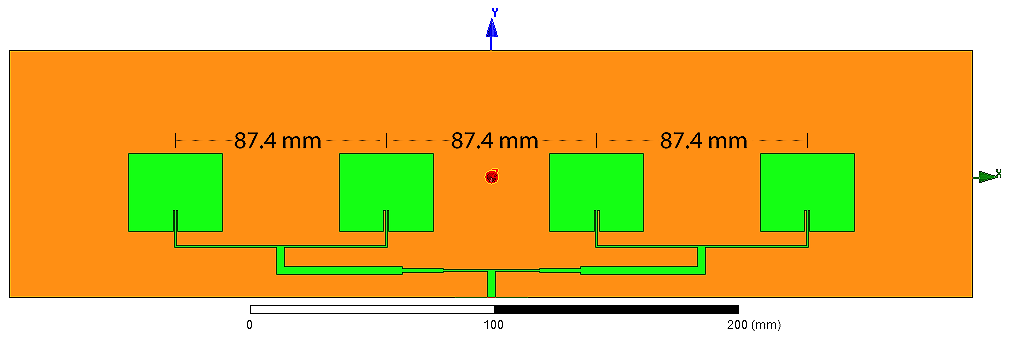
\includegraphics[width=\textwidth]{archivos/array/separacionparches}
        \caption{Ejemplo de separación entre parches para el array 4x1 a 2.4 GHz}
        \label{fig:ejemploseparación}
\end{figure}

